\section{Theoretische Grundlagen}
\label{sec:Theorie}

\subsection{Das Prinzip der Wärmepumpe}
Betrachtet man zwei Flüssigkeitsreservoire mit den Temperaturen $T_1$ und $T_2$, wobei $T_1 > T_2$ gilt, dann wird solange Wärmeenergie vom Reservoir 1 zum Reservoir 2 übertragen, bis die Temperaturdifferenz $\Delta T := T_1 - T_2$ gleich Null ist, also die Temperaturen gleich sind.
Dieser Wärmetransport lässt sich allerdings mit Hilfe einer Wärmepumpe umkehren. Unter Aufwendung von mechanischer Arbeit kann einem kälteren Reservoir Wärmeenergie entzogen werden und dem wärmeren Reservoir hinzugefügt werden.
Eine Kenngröße für die Effizienz einer Wärmepumpe ist die Güteziffer $\upnu$ (auch effektive Leistungszahl \cite{geschke}). Im Folgenden soll nun ein Ausdruck für die effektive Leistungszahl hergeleitet werden.

Die Wärmepumpe wird idealisierend als abgeschlossenes System aufgefasst.
Demnach gilt nach dem 1. Hauptsatz der Thermodynamik, dass die von einem Transportmedium an das Reservoir 1 übertragene Wärmemenge $Q_1$ gleich der Summe der vom Reservoir 2 entzogenen Wärmemenge $Q_2$ und der verrichteten Arbeit $A$ ist. Also gilt:
\begin{equation}
	\label{eqn:dQ}
	Q_1 = Q_2 + A
\end{equation}
Offensichtlich ist eine Wärmepumpe umso effizienter, wenn eine möglichst kleine mechanische Arbeit für eine möglichst große übertragene Wärmemenge $Q_1$ benötigt wird. Daher wird die Güteziffer $\upnu$ wie folgt definiert:
\begin{equation}
	\label{eqn:guete}
	\upnu := \frac{Q_1}{A}
\end{equation}
Aus der Annahme, dass die Wärmepumpe als abgeschlossenes isoliertes System angenommen wird, ergibt sich für die Entropieänderung $\symup{d}S$ des Systems
\begin{equation}
	\label{eqn:entropie}
	\symup{d}S = \frac{Q_1}{T_1} - \frac{Q_2}{T_2}
\end{equation}
Die Entropieänderung eines isolierten Systems ist gleich Null, wenn die Wärmeübertragung reversibel verläuft.
Ein reversibler Umwandlungsprozess entspricht der Annahme, dass während der Wärmeübertragung die Temperaturen $T_1$ und $T_2$, sowie die zugehörigen Drücke $p_b$ und $p_a$ konstant bleiben. Der Prozess müsste also unendlich langsam verlaufen.
Dies muss erfüllt sein, damit die vom Transportmedium aufgenommene Energie jederzeit in einem umgekehrtem Prozess wieder zurückgewonnen werden kann \cite{Anleitung}.

Aus den Gleichungen \eqref{eqn:dQ}, \eqref{eqn:guete} und \eqref{eqn:entropie} erhält man nun für die Güteziffer den Ausdruck:
\begin{equation}
	\label{eqn:gueteneu}
	\upnu = \frac{Q_1}{A} = \frac{T_1}{T_1 - T_2}
\end{equation}
Allerdings gilt Gleichung \eqref{eqn:gueteneu} nicht für den realen irreversiblen Fall.
Dann ist nämlich $\symup{d}S > 0$ und es gilt für die reale Güteziffer:
\begin{equation}
	\upnu_{real} < \frac{T_1}{T_1 - T_2}
\end{equation}
Die Wärmepumpe arbeitet also umso effektiver, je kleiner die Temperaturdifferenz $\Delta T$ ist.

Verwendet wird die Wärmepumpe, um preiswert zu heizen.
Wird mechanische Arbeit unmittelbar in Wärme umgewandelt, ist die übertragene Wärmemenge höchstens so groß wie die aufgewendete Arbeit $A$.
Mit Hilfe einer Wärmepumpe kann Wärmeenergie allerdings viel effektiver übertragen werden. Es gilt:
\begin{equation}
	Q_{1_{real}} < A \frac{T_1}{T_1 - T_2}
\end{equation}

\newpage %included because Latex moved included figure to an extra page which was ugly as f*ck. If u know something smarter to prevent latex doing cheesy formatting, please rewrite
\subsection{Die Arbeitsweise einer Wärmepumpe}

\subsection{Versuchsaufbau}
\label{sec:Versuchsaufbau}
%\begin{figure}
%	\centering
%	\caption{Schematische Darstellung des Versuchsaufbaus \cite{anleitung}.}
%	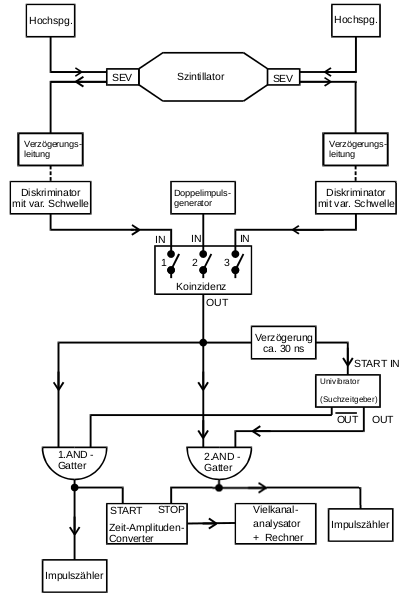
\includegraphics{Bilder/aufbau.png}
%	\label{fig:aufbau}
%\end{figure}
%
%\begin{figure}
%	\centering
%	\caption{Schematische Darstellung der Quelle zur Erzeugung radioaktiven Isotopen \cite{anleitung}.}
%	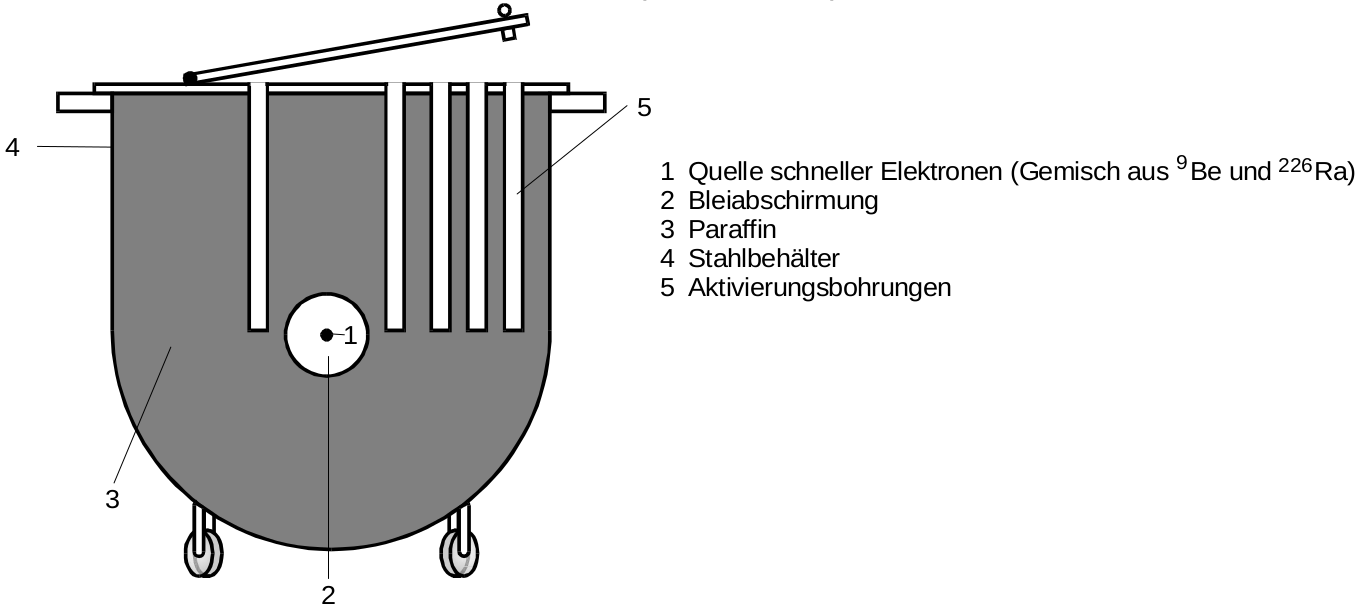
\includegraphics{content/toepfchen.png}
%	\label{fig:kochen}
%\end{figure}
%
Der Versuchsaufbau -- wie in Abbildung \ref{fig:aufbau} dargestellt -- besteht im Wesentlichen 
aus einem zerfallenden radioaktiven Isotop und einem Geiger-Müller-Zählrohr, welches die 
zerfallenden Kerne misst.
Das Geiger-Müller-Zählrohr ist entspricht einer mit Gas gefüllten Röhre. Trifft ein $\beta$-
oder $\gamma$- Teilchen auf ein Gasteilchen wird dieses ionisiert und kann aufgrund einer
anliegenden Spannung an der Röhre gemessen werden.
Dabei werden die gemessenen Zerfälle pro Messzeitintervall, welches am Zeitgeber einstellbar 
ist, an den Zählern 1 und 2 angezeigt. Nach jedem Messvorgang wird der Zähler umgeschaltet und 
der vorherige Wert auf dem aktuellen Zähler wird überschrieben. Der Versuchsaufbau ist mit
einer Blei-Abschirmung ausgestattet um die radioaktive Strahlung abzuschirmen.

Zur Erzeugung der radioaktiven Isotope wird das Objekt in Abbildung \ref{fig:kochen} verwendet.
Hierbei werden stabile Kerne mit niederenergetischen Neutronen beschossen. 
Da die Neutronen ihre Energie durch elastische Stöße an die Kerne übergeben und die maximale
Energie bei gleichen Massen der Stoßpartner erreicht wird, werden die Neutronen in einem 
Paraffinmantel gebremst, bis sie die optimale Energie besitzen.



\subsection{Bestimmung von Kenngrößen einer realen Wärmepumpe}

Bei einer Wärmepumpe sind drei Kenngrößen von besonderer Bedeutung.
\begin{enumerate}
		\item Die Güteziffer $\upnu$
		\item Der Massendurchsatz
		\item Die mechanische Kompressionsleistung $N_{mech}$
\end{enumerate}



\subsubsection {Güteziffer}
\label{sec:gueteziffer}
Für die Güteziffer gilt $\upnu = \frac{Q_1}{A}$. Mit der Kompressorleistung $N$ in einem Zeitintervall $\Delta t$ ergibt sich für die Güteziffer:
\begin{equation}
	\upnu = \frac{\Delta Q_1}{\Delta t N}
\end{equation}
Wegen dem Zusammenhang $C = \frac{\Delta Q_1}{\Delta T_1}$ (Wärmekapazität C) erhält man:
\begin{equation}
	\label{eqn:gueteziffer}
	\upnu = (m_1 c_W + m_k c_k) \frac{\Delta T_1}{\Delta t N}
\end{equation}
Wobei $m_1 c_W$ der Wärmekapazität des Reservoirs 1 und $m_k c_k$ der Wärmekapazität der Kupferschlange und des Eimers entspricht.

\subsubsection {Massendurchsatz}
\label{sec:massendurchsatz}
Für die vom Reservoir 2 abgegebene Wärmemenge $\Delta Q_2$ pro Zeitintervall $\Delta t$ gilt analog zu \ref{sec:gueteziffer}
\begin{equation}
	\frac{\Delta Q_2}{\Delta t} = (m_2 c_W + m_k c_k) \frac{\Delta T_2}{\Delta t}
\end{equation}
mit der Wärmekapazität des Reservoirs 2 $m_2 c_W$.
Die Wärmeabgabe wird durch die Verdampfung des Transportmediums realisiert.
Da die Verdampfungswärme $L$ pro Gramm definiert wurde, ist die abgegebene Wärmemenge $Q_2 = L \Delta m$. Damit ergibt sich für den Massendurchsatz mit gegebenem $L$:
\begin{equation}
	\label{eqn:massendurchsatz}
	\frac{\Delta m}{\Delta t} = \frac{\Delta Q_2}{L \Delta t}
\end{equation}



\subsubsection {Mechanische Kompressorleistung}
\label{sec:kompressorleistung}
Wird das Volumen $V_a$ des Transportmediums auf das Volumen $V_b$ komprimiert, so muss der Kompressor die Kompressionsarbeit $A_{Kompression}$ verrichten. Es gilt:
\begin{equation}
	A_{Kompression} = -\int_{V_a}^{V_b} p \symup{d}V
\end{equation}
Nun soll eine adiabatische Kompression betrachtet werden - es soll also keine Wärme mit der Umgebung ausgetauscht werden.
Dann gilt die Poissonsche Gleichung und man erhält für die Kompressionsarbeit $A_{Kompression}$:
\begin{equation}
	-p_a V_a^{\kappa} \int_{V_a}^{V_b} V^{-\kappa} \symup{d}V = \frac{1}{\kappa - 1} (p_b \sqrt[\kappa]{\frac{p_a}{p_b}} - p_a) V_a
\end{equation}
Dabei ist $\kappa := \frac{c_p}{c_V}$, wobei $c_p$ die Wärmekapazität des Transportmediums bei konstantem Druck $p$ und $c_V$ die Wärmekapazität bei konstantem Volumen $V$ ist.

Man verwende nun, dass $N_{mech} = \frac{\Delta A_m}{\Delta t}$ und $\Delta V_a = \frac{\Delta m}{\rho}$ ist und somit ergibt sich schließlich für die Kompressorleistung $N_{mech}$:
\begin{equation}
	\label{eqn:kompressorleistung}
	N_{mech} = \frac{1}{\kappa - 1} (p_b \sqrt[\kappa]{\frac{p_a}{p_b}} - p_a) \frac{1}{\rho} \frac{\Delta m}{\Delta t}
\end{equation}
Zu erwähnen ist, dass die Dichte des Transportmediums $\rho$ beim Druck $p_a$ vorliegt.
